\documentclass[11pt]{article}
\usepackage[margin=0.5in]{geometry}
\usepackage{graphicx}
\usepackage{amsmath}
\usepackage{enumitem}
\usepackage{listings}
\usepackage{float}

\graphicspath{{/home/konner/Documents/Stats_170/Project/} }

\restylefloat{table}
\begin{document}

\begin{titlepage}
\begin{center}
\vspace*{8cm}

\textbf{When are our forecasts ahead better, i.e., more accurate?}

\vspace*{1.5cm}

Konner Macias

004603916
\end{center}
\end{titlepage}

\section{Introduction}

The main question we are trying to address in this paper is: \textbf{When are our forecasts ahead better, i.e., more accurate?}
\begin{enumerate}[label=(\alph*)]
\item When the only information we use is the historical information of the time series we want to forecast, and nothing else, as when using SARIMA(p,d,q)(P,D,Q) or perhaps SARIMA with garch? 
\item When the variable we want to forecast is the dependent variable in a traditional regression model and we use other information in the form of other variables that play the role of exogenous variables? Such model could also have dummies for seasonals and polynomial trends for trend. The residuals of such a model probably need to be modeled as AR or ARIMA model to account for autocorrelation. This is the approach we used when we studied gls to approach regression with autocorrelated residuals.
\item When we use information in other variables, but the variable we want to forecast is a dependent and independent variable at the same time, and so are the other variables both dependent and independent, as in VAR?
\item  When we average the forecasted values of (a), (b), (c), to obtain a “ consensus“ forecast.
\end{enumerate}
These questions always arise in practice in a number of sciences, among them economics and meteorology. Nobody would ever use a single model to make a forecast for time $t + 1$. Almost all areas that predict the future fit several models, and then they average the forecasts obtained for each future time $t + 1$ from all the models to obtain what they called the ”consensus” forecast for time $t$. Google the word “consensus forecast“ to learn more. The Blue Chip consensus forecasts of economic indicators are an example of how the many forecasting companies out there combine their forecasts into a consensus forecast.

\section{Data}
In this section, we will describe that data that we will use to answer the question posed in the introduction. The
variable that we will want to forecast is housing starts in the United States. Housing starts is considered to be a leading indicator of what might come next in the economy. If housing construction starts to flourish that should be an indication of prosperity to come, some economists think. Other information that will be used for the models that use the other variables is unemployment rate, and unemployment rate for women. The source of the data is FRED (Federal Reserve Economic Data, 
{\tt https://fred.stlouisfed.org}). The variables are observed from January 1st 1959 to August 1st 2018. We will use January 1st 1959 to August 1st 2017 as training data, to fit the model, and then we will forecast from September 1st 2017 to August 1st 2018. Below is a table which summarizes this information about the training and testing sets. 
\begin{table}[h]
\centering
\begin{tabular}{l|r|l|l|l}
Variable Name & R Name & Description and Source                                                                                                                                                                        & Training Set                                                      & Test Set                                                          
\\
\hline
HOUSTNSA      & hs     & \begin{tabular}[c]{@{}l@{}}Housing Starts: Total new privately owned housing units\\ (in thousands). Monthly. Not seasonally adjusted\\ \textbf{This is the variable we want to forecast}\end{tabular} & \begin{tabular}[c]{@{}l@{}}Jan 1, 1959\\ Aug 1, 2017\end{tabular} & \begin{tabular}[c]{@{}l@{}}Sept 1, 2017\\ Aug 1, 2018\end{tabular} \\
\hline
LNU04000002   & uw     & \begin{tabular}[c]{@{}l@{}}Unemployment rate: Women (percent)\\ Monthly. Not seasonally adjusted\end{tabular}                                                                                 & \begin{tabular}[c]{@{}l@{}}Jan 1, 1959\\ Aug 1, 2017\end{tabular} &                                                                    \\
\hline
UNRATENSA     & ur     & \begin{tabular}[c]{@{}l@{}}Civilian Unemployment Rate (percent)\\ Monthly. Not seasonally adjusted\end{tabular}                                                                               & \begin{tabular}[c]{@{}l@{}}Jan 1, 1959\\ Aug 1, 2017\end{tabular} &                                                                   
\end{tabular}
\end{table}

\section{Data description, unit roots test, volatility checking and cointegration}
\subsection{Decomposition and Seasonal Box Plot Analysis}
Here we examine all components of the time series (observed values, trend component, seasonal component, and random component)
\begin{center}
\textbf{Figure 1. Decomposition of \tt{hs}}
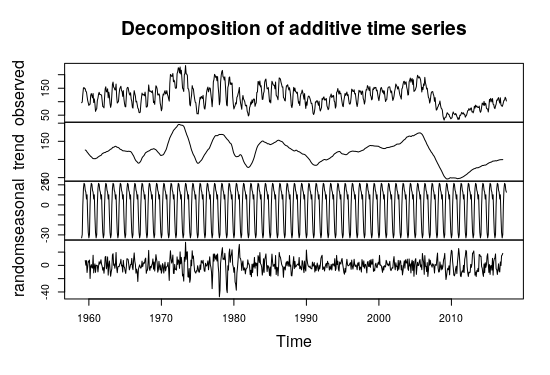
\includegraphics[scale=1]{decom-hs}
\end{center}
Looking at Figure 1, first within the observed plot, we find it difficult to depict an overall trend. This is justified by the trend component of the plot. Interestingly, the trend appears stationary until mid 2000's where it took a massive drop, most likely due to the 2008 housing crisis\footnote{https://www.americanprogress.org/issues/economy/reports/2017/04/13/430424/2008-housing-crisis/}. From the seasonal component, we notice a perfectly repeating pattern. The random component overall appears to be stationary with no obvious trends, similar to white noise. Next, let's examine the decomposition of unemployment rate for women ({\tt uw}).

\begin{center}
\textbf{Figure 2. Decomposition of \tt{uw}}
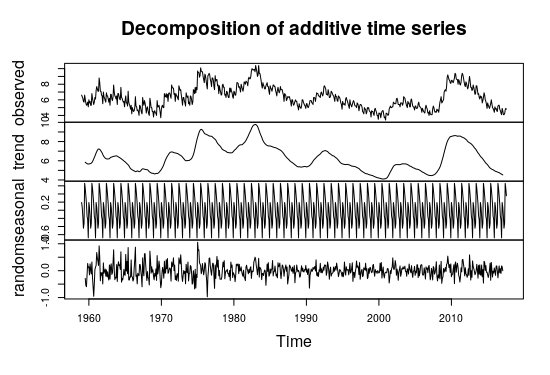
\includegraphics[scale=1]{decom-uw}
\end{center}
Looking at Figure 2, first within the observed plot, we notice periods of slow decay of unemployment followed by a sudden and quick rise. We notice that the greatest rise in terms of magnitude occured around 2008. The time plot of the data does appear to be stationary. The trend component is not regular, and only slightly indicates some stationarity. The seasonal component is obvious with a repeating patttern occuring each year. The random component appears stationary. Next, let's examine the decomposition of the overall Civilian unemployment rate ({\tt ur}).
\begin{center}
\textbf{Figure 3. Decomposition of \tt{ur}}
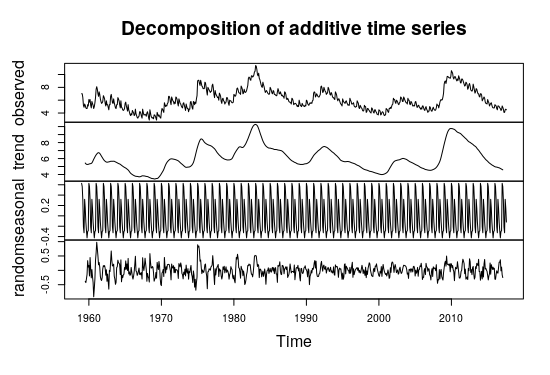
\includegraphics[scale=1]{decom-ur}
\end{center}
At first glance of Figure 3, we notice a near identical pattern as the unemployment rate for women, as it would intuitively suggest. All comments made for Figure 2 in terms of trend, seasonality, and stationarity of the random component holds. The only observable difference appears in the overall magnitude of the fluctation in the observed component, as this does not fluctuate as great as the observed component for {\tt ur}.
\\\\
Let's now examine the seasonal boxplots of each variable we are inspecting.
\begin{center}
\textbf{Figure 4.}
\\
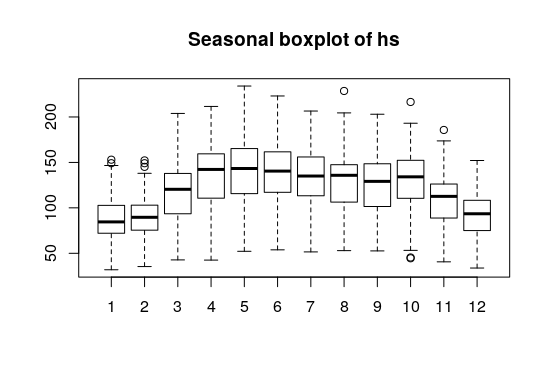
\includegraphics[scale=1]{bp-hs}
\end{center}
We notice in Figure 4 that the number of housing starts is greatest outside of the winter months. However, we notice that the IQR of these spring and summer months is very large indicating that it can very well fluctuate.

\begin{center}
\textbf{Figure 5.}
\\
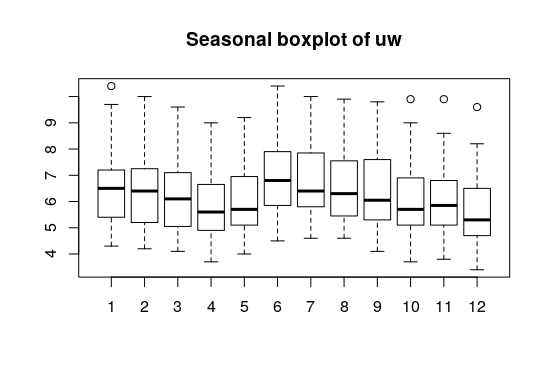
\includegraphics[scale=1]{bp-uw}
\end{center}
We notice in Figure 5 that the unemployment rate for women stays relatively the same throughout the year. We two peaks at January and June, with gradual decays occuring after those months.

\begin{center}
\textbf{Figure 6.}
\\
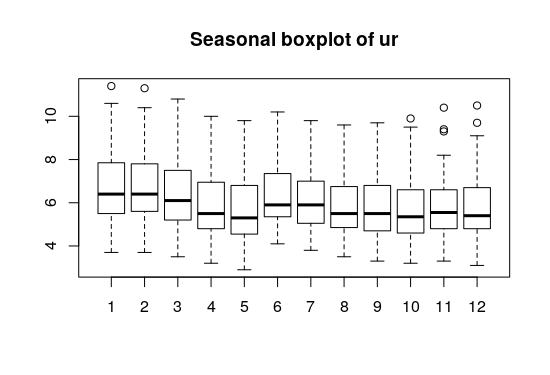
\includegraphics[scale=1]{bp-ur}
\end{center}
We notice a near identical pattern for civilian umployment rate as with women's umeployment rate. There is a slight decay after January and June.

\subsection{Unit Root, Cointegration, and Volatility Tests}
Before we begin to model, we must make sure we are not violating any underlying assumptions.
\\\\
\textbf{Unit Root Tests}
\\
To help to guarantee we are not getting a spurious regression, we perform the augumented Dickey-Fuller test which has a null hypothesis stating that a given time series $x_t$ is a random walk.
\\\\
We obtain p-values of $0.2943, 0.119, 0.09635$ for housing starts, unemployment rate for women, and civilian umeployment rate, respectively. Thus, we fail to reject the null hypothesis for all, meaning that these three time series are random walks.
\\\\
\textbf{Cointegration Tests}
\\
To verify that two series are not cointegrated and do not share an underlying stochastic trend, we perform the Phillips-Ouliaris test. The null hypothesis for this test is that the two series it is considering are NOT cointegrated.
\\\\
When comparing between each pair possible across the variables we are considering, we obtain p-values less than $0.01$, indicating that each of the variables are cointegrated with each other and share a common stochastic trend. We must take this into account when modeling, especially for the upcoming VAR model.
\\\\
\textbf{Volatility Tests}
\\
A heteroskedastic or volatile series exhibit random periods of increased variance, meaning that the variance is correlated in time even though a series may look like white noise. If this is the case for our variables, we must model the variance appropriately. Upon examination of the time plots of each of the series, we do not notice these outburst in volatility. Here, I examine the acf the data subtracted by its mean and the acf of the data subtracted by its mean squared with Figures 7 and 8.
\begin{center}
\textbf{Figure 7. ACF of (data - mean(data))}
\\
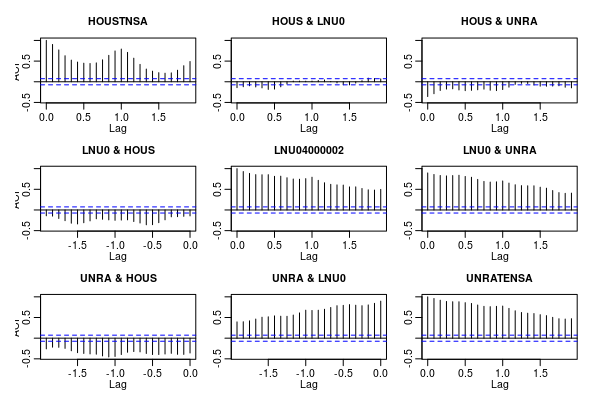
\includegraphics[scale=1]{vol1}
\end{center}

\begin{center}
\textbf{Figure 8. ACF of (data - mean(data)$)^2$}
\\
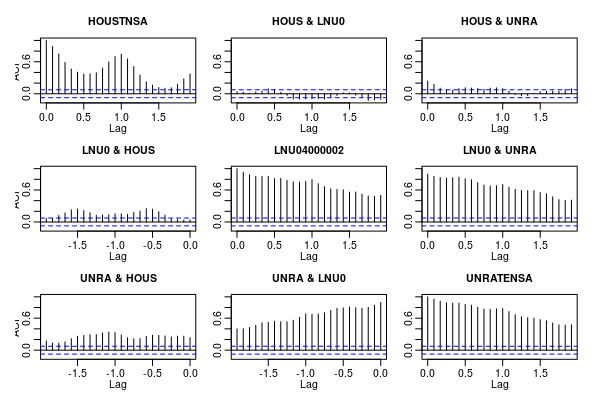
\includegraphics[scale=1]{vol2}
\end{center}

Looking at Figures 7 and 8, we notice no volatility as the spikes appears to come in a periodic fashion with no drastic outbursts.

\subsection{Autocorrelations and Cross-Correlations}
Here we wish to better understand the relationships between the variables.
\begin{center}
\textbf{Figure 9. ACFs and CCFs of the Data}
\\
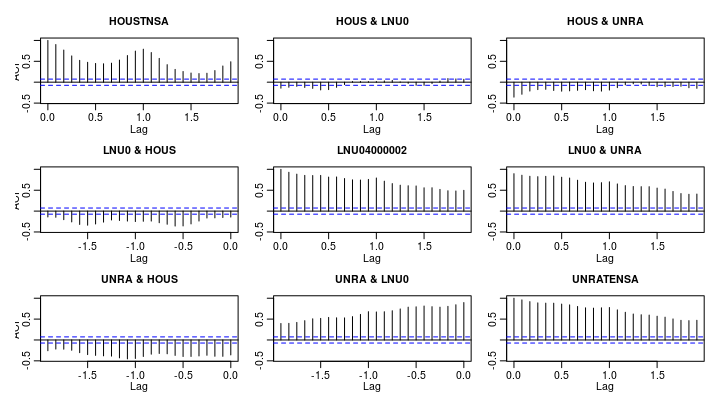
\includegraphics[scale=1]{ccf}
\end{center}
As indicated by Figure 7, we notice several significant lags when comparing in the cross-correlograms of housing starts vs. unemployment rate for women and housing starts vs. civilian unemployment rate. This indicates that unemployment rate of women and civilian unemployment affect housing starts. In fact, when comparing across each cross-correlogram, we notice that each variable affects each other as all have significant lags. Looking at the identity diagonal, we notice that we will later have to difference the data.

\section{SARIMA(p,d,q)(P,D,Q) perhaps wih garch model?}
In this section, I fit several SARIMA models to the training set of housing starts only. Before I begin, I must follow the standard procedure for appropriately identifying and fitting an ARIMA model. In section 3, we argued that the data was not volatile, thus there would be no need to run a potential GARCH with SARIMA model. Instead, a traditional SARIMA should handle the problem appropriately.
\\\\
\textbf{Transformation}
\\
Here we check whether we can transform the variance to make it more stationary allowing for us to better model the data.
\begin{center}
\textbf{Figure 10.}
\\
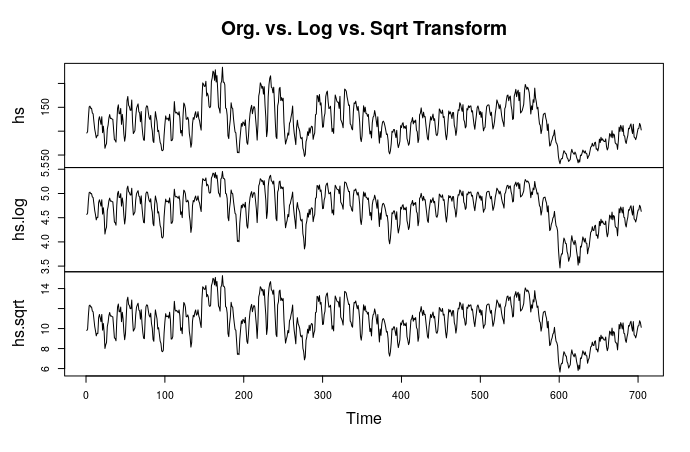
\includegraphics[scale=1]{trans}
\end{center}
Examining Figure 10, we focus on the consistency of the magnitude of fluctation across the entire time plot. The most consistent appears to be the {\tt log} transformation, though the {\tt sqrt} is close as well. We choose the log transformation over the sqrt due to its more general nature. Overall, looking at the time plot, we notice stationarity until the mid 2000s when housing starts hit a drastic decline. We call the new transformed data $hs^{\star}$. 
\\\\
\textbf{Differencing}
\\
Now we must examine whether differencing must be done to the data to make it more stationary.
\begin{center}
\textbf{Figure 11.}
\\
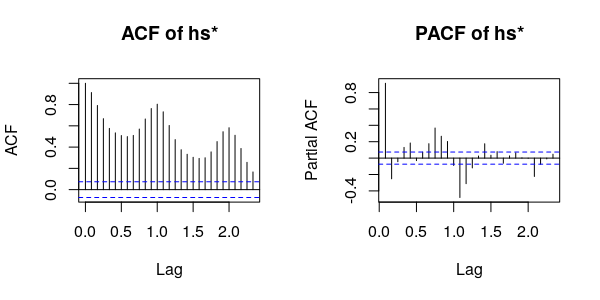
\includegraphics[scale=1]{acf-hs}
\end{center}
Figure 11 contains all statistically significant lags, but since the data itself is non-stationary, we cannot extract much information. The lags there appear to rise and falll in a pattern potentially indicating some seasonality. Next, we attempt to regularly difference.
\begin{center}
\textbf{Figure 12.}
\\
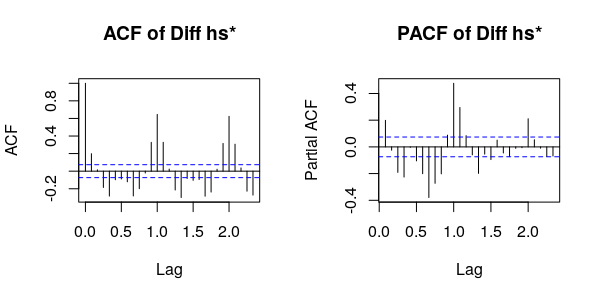
\includegraphics[scale=1]{acf-reg}
\end{center}
Figure 12 illustrates the results of regularly differencing the data. We notice that the data is still not entirely stationary as there are still several significant lags, each occuring around the end of year also indicating some underlying seasonality. Next, we take a look at solely seasonally differenced data.
\begin{center}
\textbf{Figure 13.}
\\
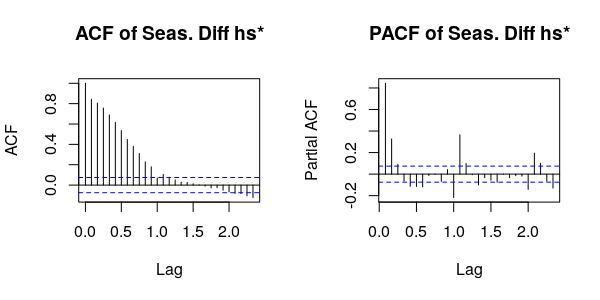
\includegraphics[scale=1]{acf-seas}
\end{center}
Looking at Figure 13, we notice that data still is not stationary yet. There appears to be a slow decay of lags in the ACF from the positive to negative direction, possibly indicating an underlying trend in the data.
\begin{center}
\textbf{Figure 14.}
\\
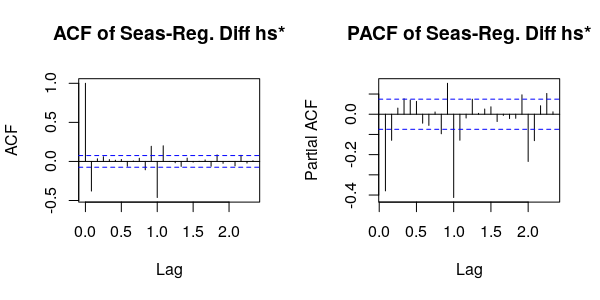
\includegraphics[scale=1]{acf-seas-reg}
\end{center}
Lastly, looking at Figure 14, we see that compared to the other ACFs, seasonally differencing the regularly differenced data proved to be the most suitable method for making the data stationary. There are still a few statistically significant lags, but this is acceptable for now as they tend to occur at the seasonal time steps. We can call this new data $hs^{\star\star}$. In combination of examination of the PACF and ACF, we obtain hints of a potential AR and MA lurking within the data. Next, we explore this further.
\\\\
\textbf{Identifying a SARIMA Model}
\\
For the sake of totality, I consider many possible combinations of models for a given SARIMA model, though we can intuitively eliminate some of the following models.
\\
We consider the following SARIMA models to best fit the data. 
\begin{center}
Model 1: $SARIMA(0,1,0)(0,1,0)_1 2$ \\
Model 2: $SARIMA(0,1,0)(1,1,0)_1 2$ \\
Model 3: $SARIMA(0,1,0)(0,1,1)_1 2$ \\
Model 4: $SARIMA(0,1,0)(1,1,1)_1 2$ \\
Model 5: $SARIMA(0,1,1)(0,1,0)_1 2$ \\
Model 6: $SARIMA(0,1,1)(1,1,0)_1 2$ \\
Model 7: $SARIMA(0,1,1)(0,1,1)_1 2$ \\
Model 8: $SARIMA(0,1,1)(1,1,1)_1 2$ \\
Model 9: $SARIMA(1,1,0)(0,1,0)_1 2$ \\
Model 10: $SARIMA(1,1,0)(1,1,0)_1 2$ \\
Model 11: $SARIMA(1,1,0)(0,1,1)_1 2$ \\
Model 12: $SARIMA(1,1,0)(1,1,1)_1 2$ \\
Model 13: $SARIMA(1,1,1)(0,1,0)_1 2$ \\
Model 14: $SARIMA(1,1,1)(1,1,0)_1 2$ \\
Model 15: $SARIMA(1,1,1)(0,1,1)_1 2$ \\
Model 16: $SARIMA(1,1,1)(1,1,1)_1 2$ 
\end{center}
Let's examine the plots of their residuals.
\begin{center}
\textbf{Figure 15.}
\\
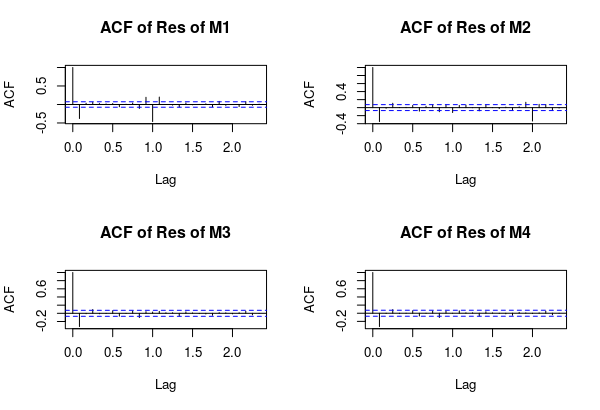
\includegraphics[scale=1]{sar1}
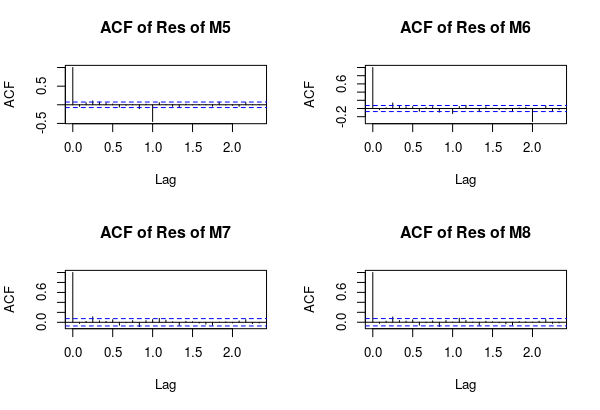
\includegraphics[scale=1]{sar2}
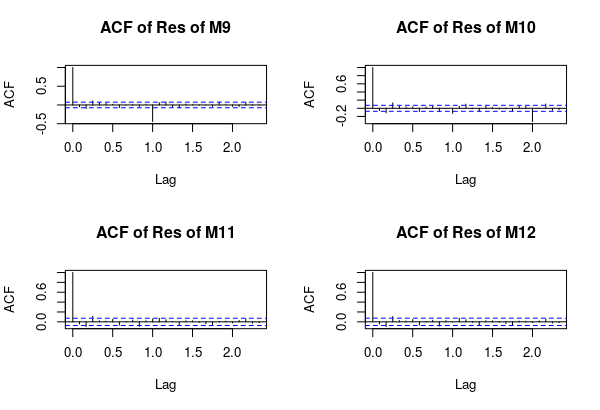
\includegraphics[scale=1]{sar3}
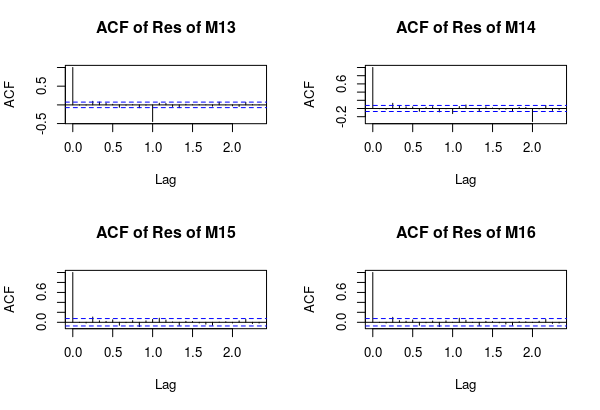
\includegraphics[scale=1]{sar4}
\end{center}
Here I decide to remove models 1,2,3,4,5,6,9,10,13, and 14 as they all contain either early statistically significant lags or additional lags around the seasonal time steps indicating that they do not do an adequate job of correctly modeling the data.
\\\\
Next, I compare the p-values of the coefficients of the remaining subset of models to check whether they are significant or not. I select against those whose model coefficients are all non-significant. With this condition of ALL being non-significant, I am unable to erase any of the remaining models from consideration. Here are my remaining models.
\begin{center}
Model 7: $SARIMA(0,1,1)(0,1,1)_1 2$ \\
Model 8: $SARIMA(0,1,1)(1,1,1)_1 2$ \\
Model 11: $SARIMA(1,1,0)(0,1,1)_1 2$ \\
Model 12: $SARIMA(1,1,0)(1,1,1)_1 2$ \\
Model 15: $SARIMA(1,1,1)(0,1,1)_1 2$ \\
Model 16: $SARIMA(1,1,1)(1,1,1)_1 2$ 
\end{center}
Let's now compare against the remaining models against several different criteria.
\begin{center}
\textbf{Figure 16.}
\end{center}
\begin{table}[h]
\centering
\begin{tabular}{|c|c|c|c|}
\hline
Model   & AIC     & $\hat{\sigma^2}$ & RMSE     \\
\hline
$SARIMA(0,1,1)(0,1,1)_1 2$ & -1342.67 & 0.008094                              & 9.223459  \\
\hline
$SARIMA(0,1,1)(1,1,1)_1 2$ & -1343.46 & 0.008061                              & 9.371128 \\
\hline
$SARIMA(1,1,0)(0,1,1)_1 2$ & -1342.67 & 0.008094                              & 9.223459 \\
\hline
$SARIMA(1,1,0)(1,1,1)_1 2$ & -1343.46 & 0.008061                              & 9.371128 \\
\hline
$SARIMA(1,1,1)(0,1,1)_1 2$ & -1342.44 & 0.008076                              & 9.195706 \\
\hline
$SARIMA(1,1,1)(1,1,1)_1 2$ & -1343.41 & 0.008042                              & 9.35449 \\
\hline
\end{tabular}
\end{table}
We see eerily similar results across the remaining models. In terms of AIC, the best model proved to be $SARIMA(0,1,1)(1,1,1)_1 2$ and $SARIMA(1,1,0)(1,1,1)_1 2$ as they had the lowest value (-$1343.46$) in comparison. In terms of $\hat{\sigma^2}$, the best model is $SARIMA(1,1,1)(1,1,1)_1 2$ since it has the lowest value ($0.008042$) in comparison. In terms of RMSE, the best model is $SARIMA(1,1,1)(0,1,1)_1 2$ as it has the lowest value ($9.195706$) in comparison. With results like these, one cannot make a particularly bad decicsion. I decide to select $SARIMA(1,1,1)(0,1,1)_1 2$ as my final model as RMSE takes precedence over the others since it is considered the most valid metric for comparing accuracy across different models. Here is the forecasting model written in polynomial form:
$$ (1 + 0.1184B)(1 - B^{12})(1 - B)y_t = (1 + (-0.8843)B^{12})(1 - 0.2433B)w_t $$
We know from above that the residuals of the model are close to white noise, so we have a valid model and thus can forecast. 
\begin{center}
\textbf{Figure 17.}
\\
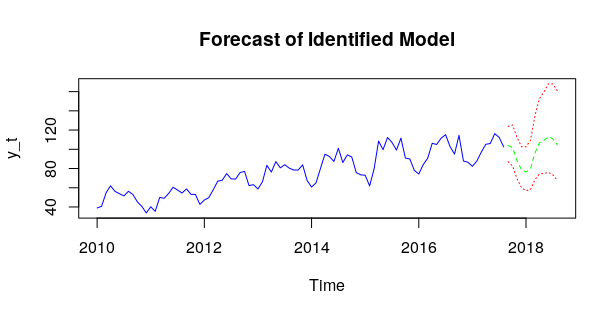
\includegraphics[scale=1]{for1}
\end{center}
Examining Figure 12, we notice that the predictions follows a similar rise and fall pattern that we noticed in previous years' data.
\section{Regression with Autocorrelated Errors}
Here I perform a classical regression, or in other words, structural equation model to model the relation between housing starts and the other independent variables ({\tt uw} and {\tt ur}). In contrast to VAR models, classical regression models require that the dependent variable ({\tt hs}) does not cause the independent variable. The direction of casuality goes only from the independent to the dependent variables and not the other way around. 
\\\\
The initial regression model of simply using only the other two variables as independent variables achieved an $R^2$ of 28.66$\%$. Next, I wanted to address the seasonally depicted in the decomposition plot of housing starts in Figure 7. Here, I create a months dummy variable which can be added into our model to help add some weight on the changing values in housing starts over the year. With this new variable added in, I achieve an $R^2$ of $42.15\%$.
\\\\
\begin{center}
\textbf{Figure 18.}
\\
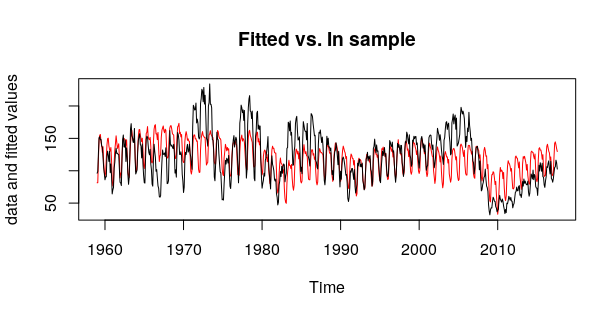
\includegraphics[scale=1]{fitIn}
\end{center}
As indicated in Figure 18, the fitted values now do a great job of rising and falling in an identical pattern as the data. In certain areas, it matches the data perfectly, however it stays more grounded across an equilibrium line compared the to the more fluctating actual data.
\\\\
We can now look at the diagnostics of our model with the other two variables and the seasonal dummy:
\begin{center}
\textbf{Figure 19.}
\\
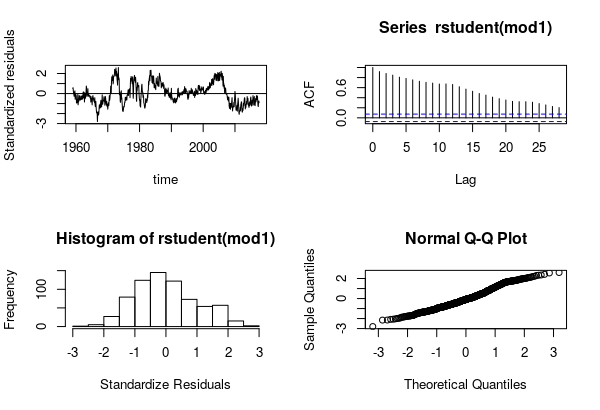
\includegraphics[scale=1]{diag}
\end{center}
Notice strong normality in the residuals judging by the shape of the histogram of the residuals and the QQ-plot indicated in Figure 19. The ACF will require further examination with its PACF.
\\\\
Here I examine the acf and pacf of the residuals for this model:
\begin{center}
\textbf{Figure 20.}
\\
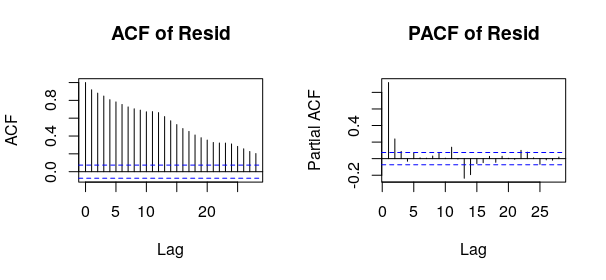
\includegraphics[scale=1]{aP}
\end{center}
Judging based on Figure 20, there is a signficant lag at the first lag of the PACF indicating an AR(1) model would be a pontential fit to this data. I then fit this model and examine the residuals.
\begin{center}
\textbf{Figure 21.}
\\
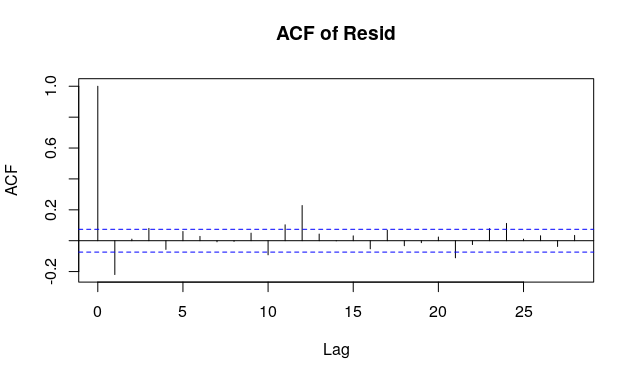
\includegraphics[scale=1]{ar1}
\end{center}
The residuals appear to resemble white noise. To incorporate the informaiton on the correlation of the residuals, I decide to utilize the {\tt gls()} function in R to add a correlation coefficient of 0.9189 which I obtained from looking at the coefficients of the AR(1) model I previously fitted. Let's examine the residuals:
\begin{center}
\textbf{Figure 22.}
\\
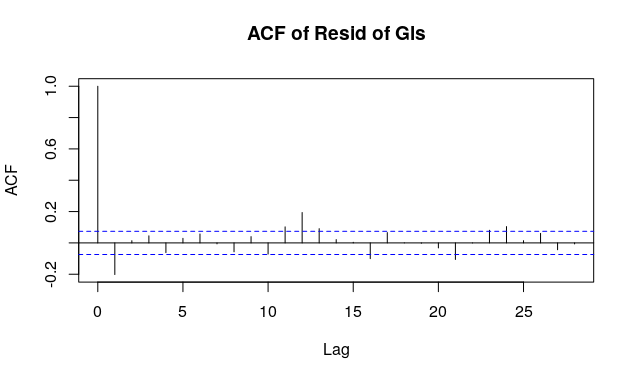
\includegraphics[scale=1]{gls1}
\end{center}
These also appear to be close to white noise.
\\\\
From here, I decide to forecast and examine the RMSE.
\begin{center}
\textbf{Figure 23.}
\\
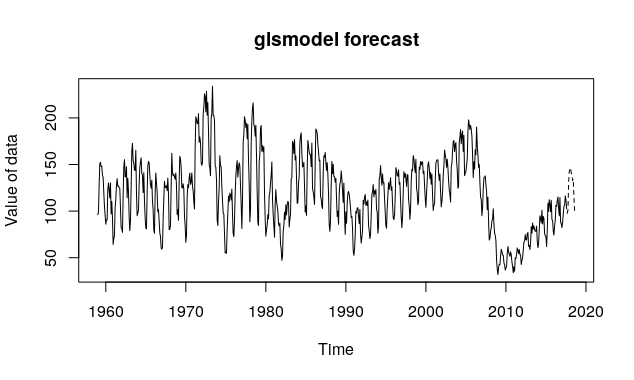
\includegraphics[scale=1]{glsFor}
\end{center}
The dashed line in Figure 23 indicates our forecast. It rises in a similar pattern but seems a little high. This particular model achieves an RMSE of 33.32007. To capture any bits of non-stochastic trend, I fit another model with a new trend component added onto the previous model.
Let's examine the residuals:
\begin{center}
\textbf{Figure 24.}
\\
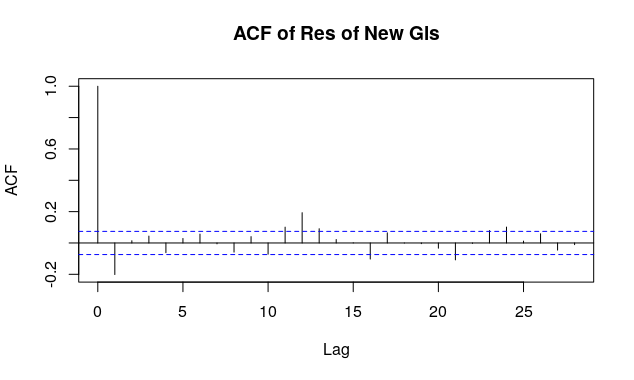
\includegraphics[scale=1]{newGls}
\end{center}
Now, let's forecast once more.
\begin{center}
\textbf{Figure 25.}
\\
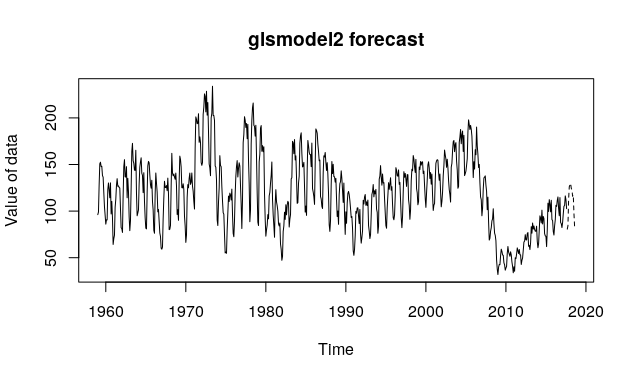
\includegraphics[scale=1]{glsFor2}
\end{center}
This appears to be further dropped down and more realistic than the previous model which did not account for any such trend. With this new model, I achieve an RMSE of 25.597, a much better result than the previous {\tt gls} model.
\section{VAR Model}
In this section, I justify the most appropriate VAR model for this data, using all the variables. Next, we observe the acf and difference to help identify a potential model. As depicted in Figure 7, the data is obviously non-stationary and needs to be differenced. In figure 26, we observe the result.
\begin{center}
\textbf{Figure 26.}
\\
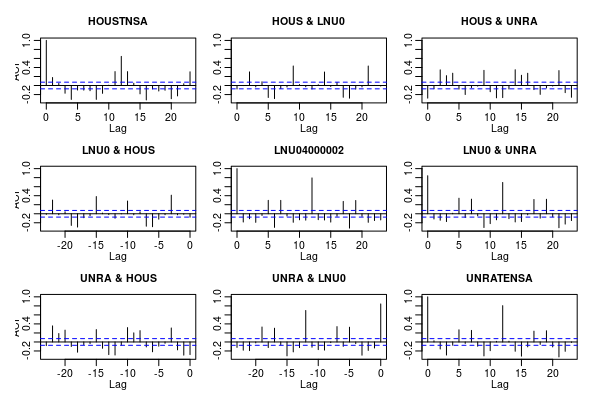
\includegraphics[scale=1]{diff}
\end{center}
Now the data and relation between the variables are more stationary. In terms of relations of one variable with the other, we notice that there is some pairwise relation between all the variables, all going both ways. We notice that the series at $t-4$ affects the other series at time $t$ then cross correlation drops, suggesting a possible p=4. This is not consistent across all relationships, and in order to verify a correct model fit, we must verify that the residuals are white noise.
\\\\
When comparing against $p=2, p=3,$ and $p=4$, we notice that $p=4$ has white noise residuals as indicated by Figure 27.
\begin{center}
\textbf{Figure 27.}
\\
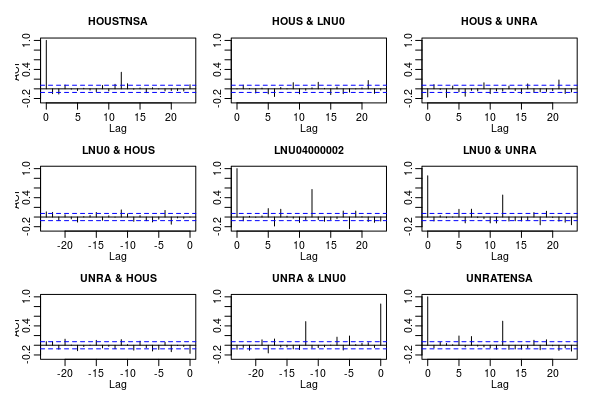
\includegraphics[scale=1]{witno}
\end{center}
We can now write our final model:
$$ hs_t = -0.007^{\star}t + 0.993hs_{t-1} + 11.685^{\star}uw_{t-1} - 13.823ur_{t-1} + 0.019hs_{t-2} - 8.533^{\star}uw_{t-2} + 21.659^{\star}ur_{t-2} - 0.058hs_{t-3} $$
$$ - 26.210^{\star}uw_{t-3} + 23.398^{\star}ur_{t-3} + 0.040hs_{t-4} + 19.203^{\star}uw_{t-4} - 26.708^{\star}ur_{t-4} $$

$$ uw_t = -0.0002^{\star}t + 0.001hs_{t-1} + 0.448^{\star}uw_{t-1} + 0.417^{\star}ur_{t-1} - 0.002hs_{t-2} + 0.087uw_{t-2} - 0.089ur_{t-2} + 0.017^{\star}hs_{t-3} $$
$$ + 0.021uw_{t-3} - 0.043ur_{t-3} + 0.0156^{\star}hs_{t-4} + 0.283^{\star}uw_{t-4} - 0.124^{\star}ur_{t-4} $$

$$ ur_t = 3.626t - 3.860^{\star}hs_{t-1} - 4.198^{\star}uw_{t-1} + 1.328^{\star}ur_{t-1} + 8.835hs_{t-2} + 2.682uw_{t-2} - 1.135ur_{t-2} + 1.409^{\star}hs_{t-3} $$
$$ + 1.434uw_{t-3} - 1.752ur_{t-3} - 1.150^{\star}hs_{t-4} + 2.614^{\star}uw_{t-4} - 4.847ur_{t-4} $$

\textbf{Who leads who?}
\\
Here, I examine the coefficients of our fitted model to check whether a series lead another. I use the rule: if $X$ has $Y$ as significant, and $Y$ does not have $X$ significant then $Y$ leads $X$.
\begin{center}
Housing Starts leads: Nothing\\
Umeployment rate for women leads: Housing starts, unemployment rate for civilians.\\
Unemployment rate for civilians leads: Housing starts, unemployment rate for women.
\end{center}
Referring back to section 3, the cointegration and unit root tests, we discovered that the variables were cointegrated with each other and each were independent random walks. Since they are cointegrated, this relation is not spurious.
\\\\
\textbf{Forecasting}
\\
Now, we will forecast the three variables for the next 12 months.
\begin{center}
\textbf{Figure 28.}
\\
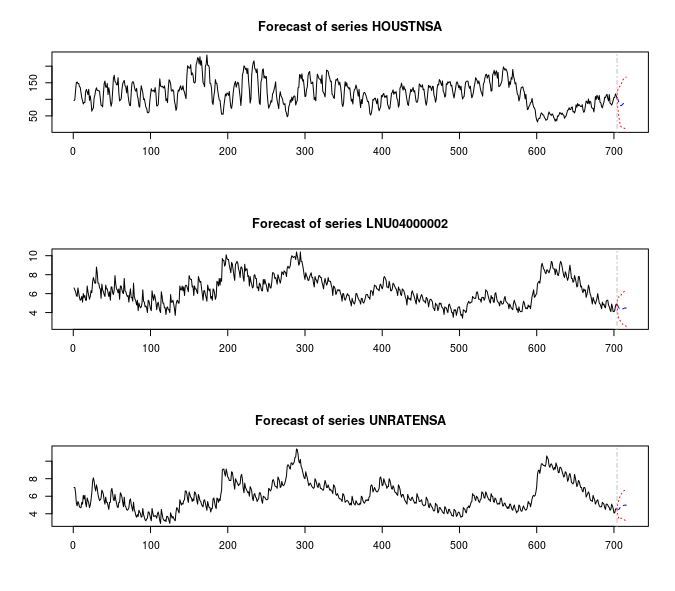
\includegraphics[scale=1]{varFor}
\end{center}
Observing Figure 28, we notice that housing starts is expected to drop and rise again. Unemployment rate for women is expected to drop and stabilize while unemployment for all citizens will gradually increase. By extracting the forecasts just for housing starts, we obtain an RMSE of $20.39057$.
\\\\
\textbf{Impulse Response Analysis}
\\
Here I perform impulse response analysis of a shock to each of the variables separately to study the dynamic relation of the whole estimated system. First, I perform a shock to housing starts and observe the system for the following 5 years.
\begin{center}
\textbf{Figure 29.}
\\
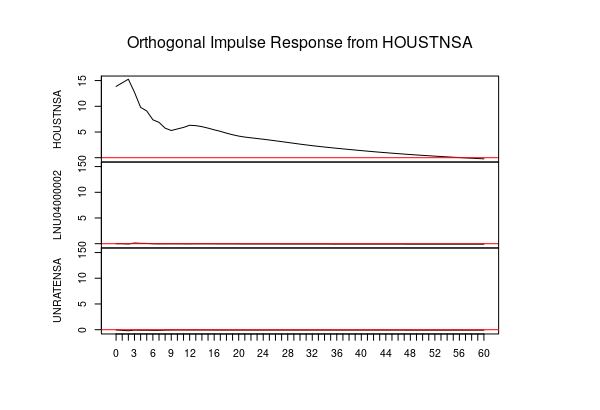
\includegraphics[scale=1]{hsShock}
\end{center}
In Figure 29, we notice that a shock to the housing starts leads to negligible effects to the others. Housing starts itself takes an initial rise than gradually falls to equilibrium over the time frame.
\begin{center}
\textbf{Figure 30.}
\\
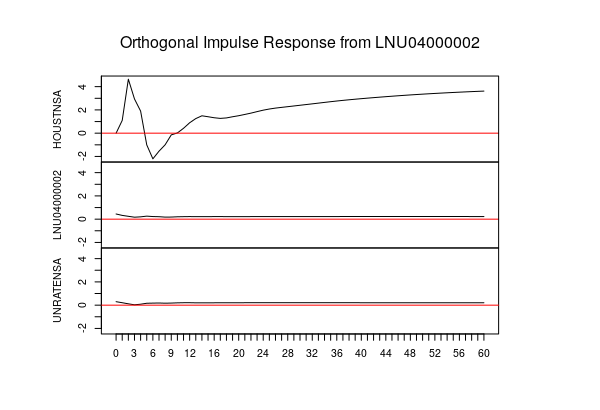
\includegraphics[scale=1]{uwShock}
\end{center}
In Figure 30, we notice that a shock to the unemployment rate for women leads to a drastic change in housing starts. Housing starts fluctuates greatly over the equilibrium and then gradually increased over the remaining years resulting in what looks to be a permanent change. The unemployment rate for civilians and women are negligibly affected over time, and share an identical pattern.
\begin{center}
\textbf{Figure 31.}
\\
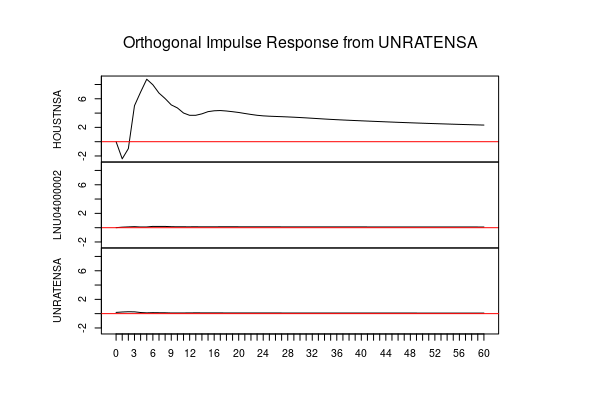
\includegraphics[scale=1]{urShock}
\end{center}
In Figure 31, we notice that a shock to the unemployment rate for civilians leads to a drastic change in housing starts. Housing initially drops below equilibrium for the first few months then immediately spikes above. After this spike, it begins to gradually fall in the direction of equilibrium. The unemployment rate for civilians and women are negligibly affected over time, and share an identical pattern.
\section{Forecasts and Conclusions}
Below, I summarize the forecasts from the three models derived in the previous sectoins for housing starts. Additionally, we present the average of these forecasts and root mean square errors.

\begin{center}
\textbf{Figure 32.}
\end{center}
\begin{table}[H]
\centering
\begin{tabular}{l|l|l|l|l|l}
\hline
Time Forecasted & SARIMA & Regression & VAR & Avg & Actual Data \\
\hline
Sept 1, 2017    & 103.81240                & 80.63850           &       101.15573 &  95.20221   &  104.4           \\
\hline
Oct 1, 2017     & 101.70848                & 84.23541           &     93.81887 &   93.25426  &   109.6          \\
\hline
Nov 1, 2017     & 88.18002                 & 112.54081           &      87.43837 &  96.05307   &   97.9          \\
\hline
Dec 1, 2017     &  78.49064                &  126.17320          &     82.66014 &  95.77466   &   81.4          \\
\hline
Jan 1, 2018     &  76.39982                &  128.02930          &     80.55905 &  94.99606   &   91.6          \\
\hline
Feb 1, 2018     &  79.62674                & 129.811112           &     82.19010 &  97.20932   &   89.7          \\
\hline
Mar 1, 2018     &  96.05839                &  124.49648          &     84.28835 & 101.61441   &   107.2          \\
\hline
Apr 1, 2018     &  106.51863               &  122.78749          &     86.78125 &  105.36246   &   117.5          \\
\hline
May 1, 2018    &  109.31832                &  115.86656          &     88.00884 &   104.39791  &   123.7          \\
\hline
June 1, 2018    &  112.96804               &  117.43530          &      88.46643 &  106.28992   &   112.0          \\
\hline
July 1, 2018    &  111.04241               &  97.75408          &     88.56794 &  99.12148   &   111.9          \\
\hline
Aug 1, 2018     &  104.63629               &  82.90668          &     88.11035 &  91.88444   &   112.6         \\
\hline 
\hline
RMSE & 9.195706 & 25.59751 & 20.39057 & 12.26739 & \\
\hline
\end{tabular}
\end{table}

As we can tell from Figure 32, the SARIMA proved to be the most accurate model in terms of prediction. However, a consensus forecast should be taughtly considered. Consensus forecasts include all possible informationfrom different modeling approaches\footnote{Introduction to Time-Series Modeling and Forecasting in Business and Economics. Garynor and Rickey. 1954.}. If one model tends to overestimate the forecast, it will be balanced out by a forecast which tends to underestimate. I good example of this was that our Regression model tended to overestimate while the VAR model tended to overestimate.
\\\\
For the most general of cases, I would recommend the consensus forecast due to the points stated above. For this particular case, I would recommend the SARIMA as it proved to be the most accurate a dependable. The RMSE compared to the other models were drastically lower and it was able to correctly understand the structure of housing start's seasonality.
\\\\
The VAR model tried to take into account the fact that the variables were cointegrated, but it errored on underestimating the forecast. Perhaps, it weighed the actions of the unemployment rates for women and civilians too much which could have decreased the overall housing rate prediction value. The model can be improved. As of now, it is simply a $p=4$ model, but perhaps further cleaning and model exploration can be done.
\\\\
The regression model performed the worst compared to the rest of the models, and is not recommended for this particular scenario.
\\\\
To address the thoughts of economists thinking that housing starts is a leading indicator, I have determined that it does not make sense. As we derived in section 6, housing starts does not lead the unemployment rate for women or civilians. After peeking at the impulse response plot after a shock was applied to housing starts, unemployment rates were not affected whatsoever. On the contrary, when either of the unemployment rates took a shock, housing starts fluctuated greatly to start the short run.
\end{document}